%************************************************
\chapter{Value Iteration with CVaR}\label{ch:vi}
%************************************************

Value iteration is a standard algorithm for maximizing expected discounted reward used in reinforcement learning. In this chapter we extend the results of \citet{chow2015risk}, who have recently proposed an approximate value iteration algorithm for CVaR MDPs. 

The original algorithm requires the computation of a linear program in each step of the value iteration procedure. Utilizing a connection between the used $\alpha \cvar_\alpha$ function and the quantile function, we sidestep the need for this computation and propose a linear-time version of the algorithm, making CVaR value iteration feasible for much larger MDPs. 

After reminding the reader of the standard value iteration algorithm, we present the original algorithm in \secref{vi:cvar}. The improved algorithm is presented in  \secref{vi:linear}, followed by section \secref{vi:experiments}, where we test the algorithm on selected environments.

%*****************************************

\section{Value Iteration}

Value iteration \citep{sutton1998reinforcement} is a well-known algorithm for computing the optimal (action-)value function and hereby finding the optimal policy. Let us remind ourselves of the Bellman optimality operator $\cT$ \eqnref{bellmanoptimalityoperator}:
\begin{equation*}
\cT Q(x,a) := \expval{ R(x, a)} + \gamma \expect\nolimits_{P} \bsquare{\max_{a' \in \cA}Q(x', a')}
\end{equation*}
or rewritten for the value function $V$
\begin{equation}
\cT V(x) := \max_a\braces{\expval{ R(x, a)} + \gamma \expect\nolimits_{P} \bsquare{V(x')}}
\end{equation}
As stated before, $\cT$ is a contraction (\secref{prelim:contraction}). This means that by repeatedly applying the operator we eventually converge to the optimal point, since we converge and the definition holds in this point. This leads to the formulation of the \textit{Value Iteration} algorithm. The only difference between theory and practice is the introduction of a small parameter $\epsilon$ that allows us to check the converge and end the algorithm when we reach a certain precision, as the contraction converges only in the limit.

See \algref{vi}.


\begin{algorithm}
\caption{Value Iteration}
\label{alg:vi}
\begin{algorithmic}
    \STATE Initialize $V$ arbitrarily (e.g. $V(x)=0$ for all $x \in \cX$)
    
	\REPEAT
	
	\STATE $v = V(x)$
	\STATE $\Delta = 0$
	
	\FOR{each $x \in \cX$}
	\STATE $V(x) = \max_a\braces{r(x, a) + \gamma\sum_{s'}p(s'|x, a)V(x')}$
	\STATE $\Delta = \max\braces{\Delta, |v-V(x)|}$
	\ENDFOR
	
	\UNTIL{ $\Delta < \epsilon$ }
	
	\STATE Output a deterministic policy $\pi \approx \pi^*$:
   	\STATE $\quad\quad \pi(x) = \argmax_a\braces{r(x, a) + \gamma\sum_{s'}p(s'|x, a)V(x')}$
\end{algorithmic}
\end{algorithm}


\section{CVaR Value Iteration}\label{sec:vi:cvar}

\citet{chow2015risk} present a dynamic programming formulation for the CVaR MDP problem \eqnref{problem}. As CVaR is a time-inconsistent measure, their method requires an extension of the state space. A Value Iteration type algorithm is then applied on this extended space and \citet{chow2015risk} proved it's convergence. 

We repeat their key ideas and results bellow, as they form a basis for our contributions presented in later sections. The results are presented with our notation introduced in \chref{prelim}, which differs slightly from the paper, but the core ideas remain the same.

\subsection{Bellman Equation for CVaR}

The results of \citet{chow2015risk} heavily rely on the CVaR decomposition theorem (Lemma 22, \citep{pflug2016time}):

\unclear{repeat the original theorems in full?}
%
\begin{equation}\label{eqn:cvardecomp}
CVaR_\alpha\bround{Z^\pi(x, a)} = \min_{\xi \in \envelope} \sum_{x'} p(x'| x, a)\xi(x') CVaR_{\xi(x')\alpha}\bround{Z^\pi(x')}
\end{equation}
%
where the risk envelope $\envelope$ coincides with the dual definition of CVaR \eqnref{envelope}.
The theorem states that we can compute the $CVaR_\alpha\bround{Z^\pi(x, a)}$ as the minimal (or worst-case) weighted combination of $CVaR_\alpha\bround{Z^\pi(x')}$ under a probability distribution perturbed by $\xi(x')$.

Note that the decomposition requires only the representation of CVaR at different confidence levels and not the whole distribution at each level, which we might be tempted to think because of the time-inconsistency issue.

\citet{chow2015risk} extend the decomposition theorem by defining the \emph{CVaR value function} $V(x, y)$ with an augmented state-space $\mathcal{X}\times\mathcal{Y}$ where $\mathcal{Y}=(0,1]$ is an additional continuous state that represents the different confidence levels.
%
\begin{equation}
V(x, y)=\max_{\pi \in \Pi_H} \cvar_{y}\bround{Z^\pi(x)}
\end{equation}
%
Similar to standard dynamic programming, it is convenient to work with with operators defined on the space of value functions. This leads to the following definition of the CVaR Bellman operator $\mathbf{T}:\mathcal{X}\times\mathcal{Y}\to\mathcal{X}\times\mathcal{Y}$:
%
\begin{equation}
\mathbf{T}V(x, y) = \max_a \bsquare{ R(x, a) + \gamma \min_{\xi \in \envelope} \sum_{x'} p(x'| x, a)\xi(x') V\bround{x', y\xi(x')}}
\end{equation}
%
or in our simplified notation:
%
\begin{equation}\label{eqn:tcvar}
\mathbf{T} CVaR_y(Z(x))=\max_a \bsquare{R(x, a) + \gamma CVaR_{y}(Z(x, a))}
\end{equation}
%
\citet{chow2015risk} further showed (Lemma 3) that the operator $\mathbf{T}$ is a contraction and also preserves the convexity of $y CVaR_t$. The optimization problem \eqnref{cvardecomp} is a convex one and therefore has a unique solution. Additionally, the fixed point of this contraction is the optimal $V^*(x, y) = \max_{\pi \in \Pi} CVaR_y (Z^\pi(x, y))$ (\citep{chow2015risk}, Theorem 4).
 
The value-function $V^*$ can then be used to extract the optimal policy $\pi^*$ of the original problem \eqnref{problem}, using the following theorem.

\begin{theorem}[Optimal Policies, Theorem 5 in \citep{chow2015risk}]\label{thm:optimalpolicy}
Let $\pi_H^*=\{\mu_0,\mu_1,\ldots\}\in\Pi_H$ be a history-dependent policy recursively defined as:
\begin{equation}\label{eqn:policy_construct}
\mu_k(h_k) = u^*(x_k, y_k),\,\,\forall k\geq 0,
\end{equation}
with initial conditions $x_0$ and $y_0=\alpha$, and state transitions
\begin{equation}\label{eqn:opt_state}
x_k\sim P(\cdot\mid x_{k-1},u^*(x_{k-1},y_{k-1})),\quad y_k = y_{k-1}\xi_{x_{k-1},y_{k-1},u^*}^*(x_k), \forall k\geq 1,
\end{equation}
where the stationary Markovian policy $u^*(x,y)$ and risk factor $\xi_{x,y,u^*}^*(\cdot)$ are solution to the  max-min optimization problem in the CVaR Bellman operator $\mathbf T[V^*](x,y)$.
Then, $\pi^*_H$ is an optimal policy for problem \eqnref{problem} with initial state $x_0$ and CVaR confidence level $\alpha$.
\end{theorem}


Naive value iteration with operator $\mathbf{T}$ is unfortunately unusable in practice, as the state space is continuous in $y$. The solution proposed in \cite{chow2015risk} is then to represent the convex $y\cvar_y$ as a piecewise linear function. 

\subsection{Value Iteration with Linear Interpolation}

Given a set of $N(x)$ interpolation points $\mathbf{Y}(x) = \braces{y_1, \dots, y_{N(x)}}$, we can interpolate the $yV(x,y)$ function on these points, i.e.
%
\begin{equation*}
\interpI_{x}[V](y)=y_iV(x,y_{i})+\frac{y_{i+1}V(x,y_{i+1})-y_iV(x,y_{i})}{y_{i+1}-y_i}(y-y_i),
\end{equation*}
%
where $y_i = \max \left\{y'\in \mathbf{Y}(x) : y' \leq y\right\}$
The interpolated Bellman operator $\mathbf{T}_\interpI$ is then also a contraction and has a bounded error (\citep{chow2015risk}, Theorem 7). 
\todo{bounded -> linear in $\theta$}
%
\begin{equation}\label{eqn:linearbellman}
\mathbf{T}_\interpI V(x, y) = \max_a \bsquare{ R(x, a) + \gamma \min_{\xi \in \envelope} \sum_{x'} p(x'| x, a)\dfrac{\interpI_{x'} [V](y\xi(x'))}{y}}
\end{equation}
%
The full value iteration procedure is presented in \algref{cvarlinear}. 

This algorithm can be used to find an approximate global optimum in any MDP. There is however the issue of computational complexity. As the algorithm stands, the straightforward approach is to solve each iteration of \eqnref{linearbellman} as a linear program, since the problem is convex and piecewise linear, but this is not practical, as the LP computation can be demanding and is therefore not suitable for large state-spaces.

\unclear{maybe formulate the LP exactly?}

In the next section we aim to find a different way of computing the optimization problem.

\begin{algorithm}[h]
\caption{\texttt{CVaR Value Iteration with Linear Interpolation}}
\label{alg:cvarlinear}
1: \textbf{Given:}
\begin{itemize}
%\item An interpolation error bound $\epsilon>0$ for small CVaR thresholds.
\item $N(x)$ interpolation points $\mathbf{Y}(x)  = \left\{y_1,\dots,y_{N(x)}\right\} \in [0,1]^{N(x)}$ for every $x\in \mathcal X$ with $y_i<y_{i+1}$, $y_1=0$ and $y_{N(x)}=1$.
%, $y_2 = \min_{x',a}\{ P(x'|x,a):P(x'|x,a)\neq 0\}$
%\item An interpolation function $\interpI_{x}[V](y;\interpY(x))$ for $yV(x,y)$ for any arbitrary value function $V$.
\item Initial value function $V_0(x,y)$ that satisfies:
\begin{enumerate}
\item $yV_0(x,y)$ is convex in $y$ for all $x$
\item $yV_0(x,y)$ is continuous in $y$ for all $x$
\end{enumerate}
 %where $V_0(x,y)=0$ at $y<0$.
\end{itemize}
2: Repeat until convergence:
\begin{itemize}
%\item Update the smallest non-zero grid $y_2$ in $\interpY(x)$ by choosing it to satisfy $\max_{x\in\mathcal X, y\in \mathbf I_2(x)}|V_0(x,y_2)-V_0(x,y)|\leq\epsilon$, where the interpolation based Bellman operator $ \bellint$ is given by
%  \[
%\hspace{-0.5in}  \bellint[V](x,y) =
% \min_{a\in\mathcal A}\left[C(x,a)+\gamma\max_{\xi\in \U_{\text{CVaR}}(y, P(\cdot|x,a))}\sum_{x'\in\mathcal X}\frac{\interpI_{x'}[V](y\xi(x');\interpY(x'))}{y}P(x'|x,a)\right].
%   \]
\item For each $x \in \mathcal X$ and each $y_i\in \mathbf{Y}(x)$, update the value function estimate as follows:
  \begin{equation*}
   V_{k+1}(x,y_i)= \mathbf{T}_\interpI[V_k](x,y_i),
  \end{equation*}
  \end{itemize}
3: Set the converged value iteration estimate as $\widehat{V}^*(x,y_i)$, for any $x\in\mathcal X$, and $ y_i\in\mathbf{Y}(x)$.
\end{algorithm}


%*****************************************

\section{Efficient computation using quantile representation}\label{sec:vi:linear}

We present our original contributions in this section. We first describe a connection between the $y\cvar_y$ function and the quantile function of the underlying distribution. We then use this connection to formulate a faster computation of the value iteration step, resulting in the first linear-time algorithm for solving CVaR MDPs with bounded error.

\begin{lemma}\label{thm:varcvarconnection}
Any discrete distribution has a piecewise linear and convex $y\cvar_y$ function. Similarly, any piecewise linear convex function can be seen as representing a certain discrete distribution.
\\
Particularly, the integral of the quantile function is the $y\cvar_y$ function
\begin{equation}\label{eqn:varcvarintegration}
y\cvar_y(Z) = \int_0^y VaR_\beta(Z) \dt \beta
\end{equation}
and the derivative of the $y\cvar_y$ function is the quantile function
\begin{equation}\label{eqn:varcvarderivation}
\dfrac{\partial}{\partial y} y \cvar_y(Z) = VaR_y(Z)
\end{equation}
\end{lemma}

\begin{proof}
The fact that discrete distributions have has already been shown by \citet{rockafellar2000optimization}.
\\
According to definition \eqnref{cvardef} we have
\begin{equation*}
y\cvar_y(Z) = y\dfrac{1}{y}\int_0^y VaR_\beta(Z) \dt \beta = \int_0^y VaR_\beta(Z) \dt \beta
\end{equation*}
by taking the $y$ derivative, we have
\begin{equation*}
\dfrac{\partial}{\partial y} y \cvar_y(Z) = \dfrac{\partial}{\partial y} \int_0^y VaR_\beta(Z) d\beta = VaR_y(Z)
\end{equation*}
\end{proof}

You can get some intuition from \figref{cvarvisual}, where the integral-derivation relationship is clearly visible.

According to Lemma \ref{thm:varcvarconnection}, we can reconstruct the $y\cvar_y$ from the underlying distribution and vice-versa. We utilize the fact that the conversion is linear in the number of probability atoms to formulate a fast way of computing the $\mathbf{T}_\interpI$ operator.

\begin{figure}
\center
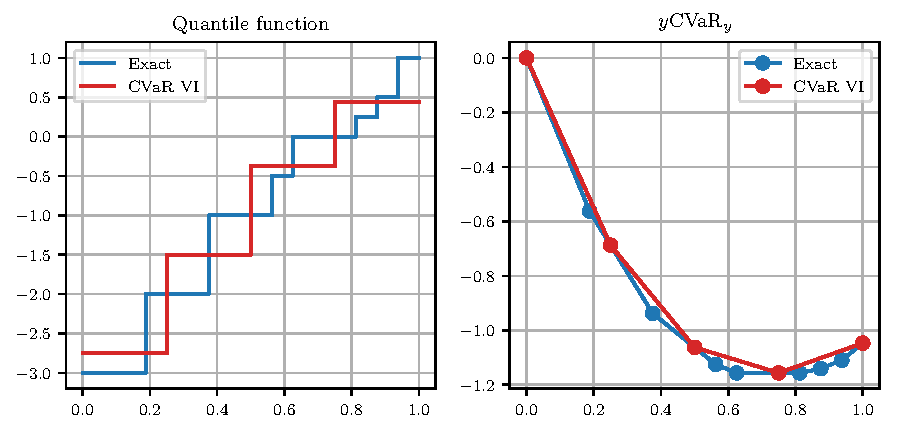
\includegraphics[width=\linewidth]{gfx/cvar_visualized.pdf}
\caption{Comparison of a discrete distribution and it's approximation according to the CVaR linear interpolation operator.}
\label{fig:cvarvisual}
\end{figure}

\subsection{CVaR Computation via Quantile Representation}

We propose the following procedure: instead of using linear programming for the CVaR computation, we use the underlying distributions represented by the $\alpha CVaR_\alpha$ function to compute CVaR.

The computation of CVaR of a discrete probability mixture is a linear-time process as we show bellow. The general steps of the computation are as follows

\begin{enumerate}
\item transform $y \cvar_y$ of each possible state transition to a discrete probability distribution function using \eqnref{varcvarderivation}
\item combine these to to a distribution representing the full state-action distribution
\item compute $y \cvar_y$ for all atoms using \eqnref{varcvarintegration}
\end{enumerate}
See \figref{cvarcomputation} for a visualization of the procedure.

\begin{figure}
\center
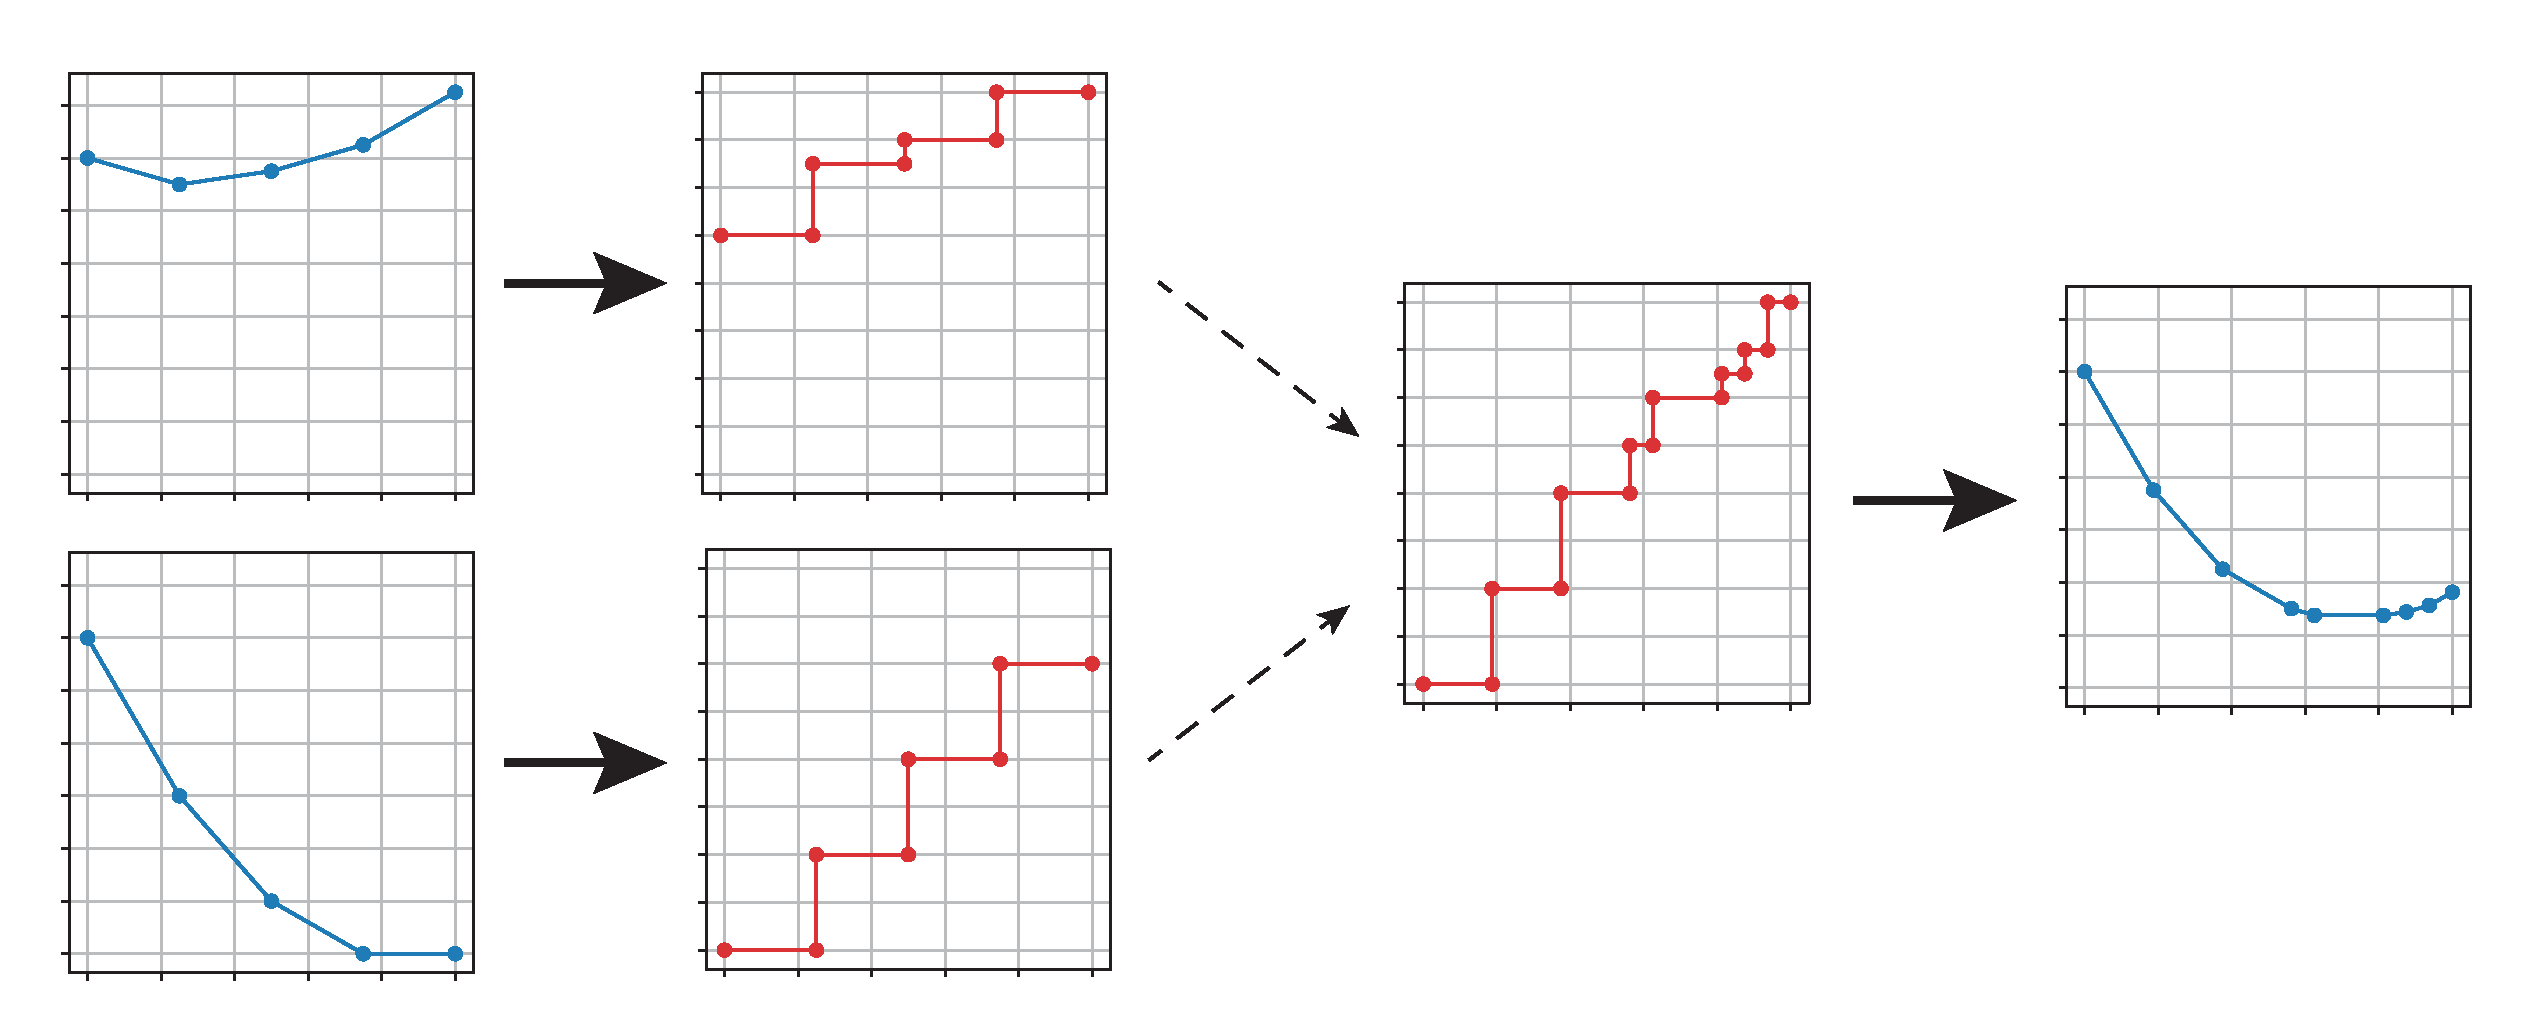
\includegraphics[width=\linewidth]{gfx/cvar_vi_conversion.pdf}
\caption{Visualization of the CVaR computation for a single state and action with two transition states. Thick arrows represent the conversion between $\ycvary$ and the quantile function.}
\label{fig:cvarcomputation}
\end{figure}

\todo{show the linearity}
\unclear{show an example computation?}

\unclear{proof necessary? also, maybe it is already in the $\xi$ proof}


%\begin{algorithm}
%\caption{CVaR computation}
%
%\begin{multicols}{2}
%
%\begin{algorithmic}
%    \STATE \textbf{input} $\alpha, x_t, \pi_\text{old}, \gamma$
%    \WHILE{$x_t$ is not terminal}
%    	\STATE $a = \text{arg}\max_a CVaR_\alpha(Z(x_t, a))$
%		\STATE $s = VaR_\alpha(Z(x_t, a))$
%		\columnbreak
%
%    	\STATE $x_t, r_t = \text{envTransition}(x_t, a)$
%    	\STATE $\alpha = F_{Z(x_t, \pi_\text{old}(x_t))}\left(\dfrac{s - r}{\gamma}\right) $ \textcolor{gray}{\# $VaR_\alpha(Z(x_t, \pi_\text{old}(x_t))) == \dfrac{s - r}{\gamma}$}
%   	\ENDWHILE
%\end{algorithmic}
%\end{multicols}
%\end{algorithm}
%
%\begin{minipage}[t]{0.5\linewidth}
%  \vspace{0pt}  
%  \begin{algorithm}[H]
%    \caption{Algo 1}
%    line 1\;
%    line 2\;
%  \end{algorithm}
%\end{minipage}%
%\begin{minipage}[t]{5cm}
%  \vspace{0pt}
%  \begin{algorithm}[H]
%    \caption{Algo 1}
%    line 1\;
%  \end{algorithm}
%\end{minipage}

\subsection{$\xi$-computation}

Similarly to \thmref{optimalpolicy}, we need a way to compute the $y_{k+1}=y_{k}\xi^*(x_k)$ to extract the optimal policy. Again, we can skip the LP computation by using the following intuition: $y_{k+1}$ is the portion of $Z(x_{k+1})$ that is present in $\cvar_{y_k}(Z(x_k))$. In the continuous case, it is the probability in $Z(x_{k+1})$ before the $\var_{y_k}(Z(x_k))$ as we show bellow.

\todo{proof for discrete distributions}

\begin{theorem}
Solution to minimization problem \eqnref{cvardecomp} can be computed without optimization by setting
\begin{equation}\label{eqn:xi-claim}
\xi ( x' ) = \dfrac{F_{x'}(F^{-1}_x(\alpha))}{\alpha} 
\end{equation}
\end{theorem}

\begin{proof}
For simplification, we work only with two states: $x'$ the actual sampled state and $\bar{x}'$ representing the other states. The equation then simplifies to

\begin{equation}\label{eqn:cvardecomp2}
\begin{split}
CVaR_\alpha(x, a)&=\min_{\xi} \, p\xi CVaR_{\xi\alpha}(x') + (1-p)\dfrac{1-p\xi}{1-p}CVaR_{\frac{1-p\xi}{1-p}\alpha}(\bar{x}')\\
&=\min_{\xi} \, p\xi CVaR_{\xi\alpha}(x') + (1-p\xi)CVaR_{\frac{1-p\xi}{1-p}\alpha}(\bar{x}')\\
\end{split}
\end{equation}

To find the min we first find the first derivative\footnote{
We used the following identities:
\begin{equation*}
\dfrac{\partial CVaR_{\alpha\xi}}{\partial \xi} = \frac{1}{\xi}VaR_{\xi\alpha}-\frac{1}{\xi}CVaR_{\xi\alpha}\quad\quad\quad
\dfrac{\partial CVaR_{\frac{1-p\xi}{1-p}\alpha}}{\partial\xi} = \frac{p}{1-p\xi}CVaR_{\frac{1-p\xi}{1-p}\alpha}	-	\frac{p}{1-p\xi}VaR_{\frac{1-p\xi}{1-p}\alpha}
\end{equation*}
} w.r.t. $\xi$

\begin{equation}
\begin{split}
\dfrac{\partial CVaR_\alpha}{\partial \xi} &= pCVaR_{\xi\alpha} + p\xi \dfrac{\partial CVaR_{\alpha\xi}}{\partial \xi} - pCVaR_{\frac{1-p\xi}{1-p}\alpha} + (1 - p\xi)\dfrac{\partial CVaR_{\frac{1-p\xi}{1-p}\alpha}}{\partial\xi}\\
&= pCVaR_{\xi\alpha} + p\xi\left[	\frac{1}{\xi}VaR_{\xi\alpha}-\frac{1}{\xi}CVaR_{\xi\alpha}	\right] - pCVaR_{\frac{1-p\xi}{1-p}\alpha} \\&\hspace*{5cm} + (1-p\xi)\left[	\frac{p}{1-p\xi}CVaR_{\frac{1-p\xi}{1-p}\alpha}	-	\frac{p}{1-p\xi}VaR_{\frac{1-p\xi}{1-p}\alpha}\right]\\
&= pCVaR_{\xi\alpha} + pVaR_{\xi\alpha} - pCVaR_{\xi\alpha} - pCVaR_{\xi\alpha} - pCVaR_{\frac{1-p\xi}{1-p}\alpha} \\&\hspace*{5cm} + CVaR_{\frac{1-p\xi}{1-p}\alpha} - pVaR_{\frac{1-p\xi}{1-p}\alpha}\\
&= pVaR_{\xi\alpha} - pVaR_{\frac{1-p\xi}{1-p}\alpha}
\end{split}
\end{equation}

By setting the derivative to 0 (to find the min), we get
\begin{equation}\label{eqn:varvar}
VaR_{\xi\alpha}(x')= VaR_{\frac{1-p\xi}{1-p}\alpha}(\bar{x}')
\end{equation}

By inserting claim \eqnref{xi-claim} into \eqnref{varvar} we get the symmetrical claim
\begin{equation}
\dfrac{1-p\xi}{1-p} = \xi(\bar{x}') = \dfrac{F_{\bar{x}'}(F^{-1}_x(\alpha))}{\alpha}
\end{equation}

We rewrite \eqnref{cvardecomp2} as (assuming $\xi$ is the minimum point)

\begin{equation}
\begin{split}
\frac{1}{\alpha} \int_0^\alpha F^{-1}_{x}(t)dt &= p\xi \frac{1}{\xi\alpha} \int_0^{\xi\alpha} F^{-1}_{x'}(t)dt + (1-p\xi)\frac{1-p}{(1-p\xi)\alpha} \int_0^{\frac{1-p\xi}{1-p}\alpha} F^{-1}_{\bar{x}'}(t)\\
&=p \frac{1}{\alpha} \int_0^{\xi\alpha} F^{-1}_{x'}(t)dt + (1-p)\frac{1}{\alpha} \int_0^{\frac{1-p\xi}{1-p}\alpha} F^{-1}_{\bar{x}'}(t)
\end{split}
\end{equation}

This must also hold if we multiply both sides by $\alpha$
\begin{equation}
\int_0^\alpha F^{-1}_{x}(t)dt = p\int_0^{\xi\alpha} F^{-1}_{x'}(t)dt + (1-p)\int_0^{\frac{1-p\xi}{1-p}\alpha} F^{-1}_{\bar{x}'}(t)
\end{equation}
And we take derivations w.r.t. $\alpha$ of both sides
\begin{equation}
F^{-1}_{x}(\alpha) = p\xi F^{-1}_{x'}(\xi\alpha) + (1-p\xi) F^{-1}_{\bar{x}'}(\frac{1-p\xi}{1-p}\alpha)
\end{equation}


By inserting \eqnref{xi-claim} we get
\begin{equation}
\begin{split}
 p\xi F_{x'}^{-1}(\xi\alpha) + (1-p)\xi_2 F_{\bar{x}'}^{-1}\left(\xi_2\alpha\right) &= p\xi F_{x'}^{-1}(F_{x'}(F^{-1}_x(\alpha))) + (1-p\xi) F_{\bar{x}'}^{-1}\left(F_{\bar{x}'}(F^{-1}_x(\alpha))\right)\\
 &= p\xi F_x^{-1}(\alpha) + (1-p\xi)F_x^{-1}(\alpha) = F_x^{-1}(\alpha)
\end{split}
\end{equation}

We've shown that the proposed solution \eqnref{xi-claim} satisfies the minimization constraint \eqnref{varvar} (= is a minimal point) and satisfies the dual decomposition \eqnref{cvardecomp}. (This has been shown only in the differentiated form )

\end{proof}


%*****************************************



\section{Experiments}\label{sec:vi:experiments}

\todo{$|\mathcal{X}|\sim 1M$ tabular environment}

\todo{get matlab code from tamar}

\subsection{Cliffworld}

\section{Summary}


%*****************************************
%*****************************************
%*****************************************
%*****************************************
%*****************************************



